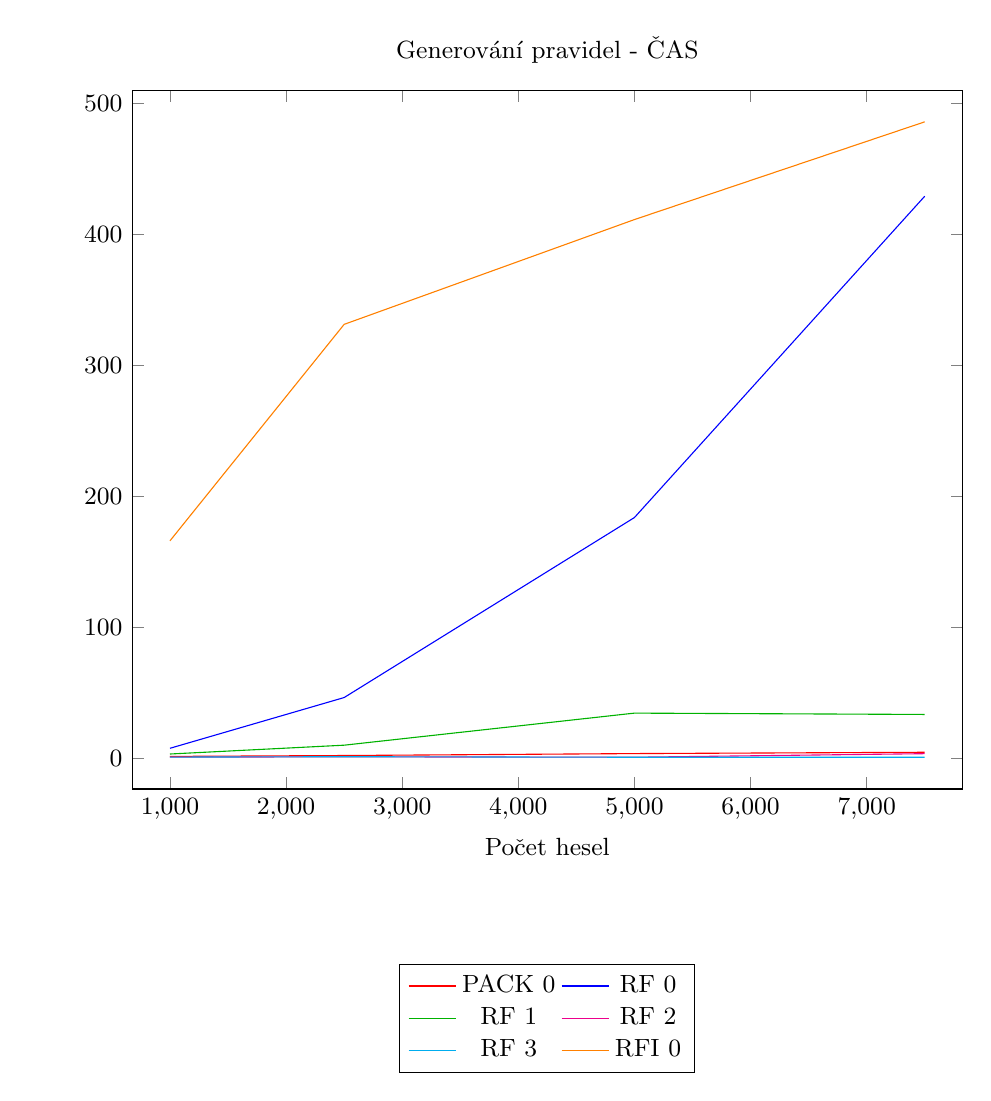
\begin{tikzpicture}
  \begin{axis}[
    width=\linewidth, 
    every axis/.append style={font=\small},
    title={Generování pravidel - ČAS},
    xlabel={Počet hesel},
    ylabel={\phantom{Čas [s]}},
    legend style={
      at={(0.5,-0.25)},
      anchor=north,
      legend columns=2,
    },
    enlargelimits=0.05,
    scaled y ticks = false,
    scaled x ticks = false,
    cycle list={
     {red},
     {blue},
     {green!70!black},
     {magenta},
     {cyan},
     {orange},
     {violet},
     {purple},
     {gray},
     {darkgray}%
    }
    ]
    
    \addplot coordinates {
      (1000, 1.74) 
      (2500, 2.43) 
      (5000, 3.91) 
      (7500, 4.91) 
      }; % PACK 0
    
    \addplot coordinates {
      (1000, 7.95) 
      (2500, 46.68) 
      (5000, 184.07) 
      (7500, 429.32) 
      }; % RF 0
    
    \addplot coordinates {
      (1000, 3.58) 
      (2500, 10.32) 
      (5000, 34.79) 
      (7500, 33.77) 
      }; % RF 1
    
    \addplot coordinates {
      (1000, 1.22) 
      (2500, 1.42) 
      (5000, 1.13) 
      (7500, 3.84) 
      }; % RF 2
    
    \addplot coordinates {
      (1000, 1.22) 
      (2500, 1.52) 
      (5000, 1.11) 
      (7500, 1.11) 
      }; % RF 3
    
    \addplot coordinates {
      (1000, 166.32) 
      (2500, 331.52) 
      (5000, 411.5) 
      (7500, 486.1) 
      }; % RFI 0
    
    \legend{PACK 0, RF 0, RF 1, RF 2, RF 3, RFI 0}
  \end{axis}
\end{tikzpicture}